\documentclass[12pt, twoside]{article}
\input{../preamble}

\fancyhead[LE]{\thepage}
\fancyhead[RO]{\thepage}
\fancyhead[LO]{La Scuola d'Italia / Huson / IB Math: Distributions --- Solutions \\* 26 February 2026}

\begin{document}

\subsubsection*{4.16 Do Now: Normal and Binomial Distribution Practice --- Solutions}
\begin{enumerate}[itemsep=0.1cm]

%--- Problem 1 ---
\item The heights, $H$ cm, of sunflowers grown in a garden competition are normally distributed
with a mean of 148\,cm and a standard deviation of 11\,cm.

\begin{enumerate}[itemsep=0.25cm]
    \item Find $\mathrm{P}(H < 140)$. \hfill [2]
    \item Find $\mathrm{P}(135 < H < 160)$. \hfill [2]
    \item The tallest 20\% of sunflowers receive a prize. Find the minimum height, in cm,
    required to receive a prize. \hfill [2]
    \item Given that a sunflower does not receive a prize, find the probability that it is
    taller than 150\,cm. \hfill [2]
\end{enumerate}

\vfill

\begin{tikzpicture}
  \draw (0,0) rectangle (15.5,13);
  \node[anchor=north west, inner sep=0.40cm] at (0,13) {%
    \begin{minipage}[t]{14.7cm}%
      \textbf{Solutions}\\[0.4cm]
      %--- (a) with normal curve sketch to the right ---
      \begin{minipage}[t]{9.0cm}%
        \textbf{(a)}\enspace $\mathrm{normCdf}(0,\;140,\;148,\;11) = 0.23352\ldots$\\[0.1cm]
        \hspace*{2.5em}$\approx \mathbf{0.234}$%
      \end{minipage}%
      \hfill%
      \begin{minipage}[t]{4.8cm}%
        \centering
        \tikz[scale=0.72, baseline=(current bounding box.center)]{%
          \fill[gray!35]
            plot[domain=-3:-0.727,samples=30,variable=\t](\t,{exp(-\t*\t/2)})
            --(-0.727,0)--(-3,0)--cycle;
          \draw[thick] plot[domain=-3:3,samples=60,variable=\t](\t,{exp(-\t*\t/2)});
          \draw(-3.2,0)--(3.2,0);
          \draw[dashed](-0.727,0.768)--(-0.727,0);
          \foreach \xv/\lab in {-1/137, 0/148, 1/159}{
            \draw(\xv,0.05)--(\xv,-0.05);
            \node[below,font=\tiny]at(\xv,0){\lab};
          }
          \node[below,yshift=-5pt,font=\tiny]at(-0.727,0){$140$};
        }%
      \end{minipage}\\[0.4cm]
      %--- (b) ---
      \textbf{(b)}\enspace $\mathrm{normCdf}(135,\;160,\;148,\;11) = 0.74370\ldots$\\[0.1cm]
      \hspace*{2.5em}$\approx \mathbf{0.744}$\\[0.4cm]
      %--- (c) ---
      \textbf{(c)}\enspace $\mathrm{invNorm}(0.80,\;148,\;11) = 157.258\ldots$\\[0.1cm]
      \hspace*{2.5em}$\approx \mathbf{157}$ cm\\[0.4cm]
      %--- (d) two steps ---
      \textbf{(d)}\enspace $\mathrm{normCdf}(150,\;157.258\ldots,\;148,\;11) = 0.22786\ldots$\\[0.2cm]
      \hspace*{2.5em}$\dfrac{0.22786\ldots}{0.80} = 0.28482\ldots \approx \mathbf{0.285}$%
    \end{minipage}%
  };
\end{tikzpicture}

\newpage

%--- Problem 2 ---
\item A city bus arrives on time at a particular stop with probability 0.65. Over a period
of one week, the bus makes 20 scheduled arrivals. The number of times the bus arrives
on time is denoted by $X$.

\begin{enumerate}[itemsep=0.25cm]
    \item Find $\mathrm{P}(X = 13)$. \hfill [2]
    \item Find $\mathrm{P}(X \geq 15)$. \hfill [2]
    \item Find $\mathrm{E}(X)$ and $\mathrm{Var}(X)$. \hfill [2]
    \item Find the greatest integer value of $n$ such that $\mathrm{P}(X \geq n) > 0.95$. \hfill [3]
    \item Explain in the context of the problem what the value of $n$ found in \\
    part (d) represents. \hfill [1]
\end{enumerate}

\vfill

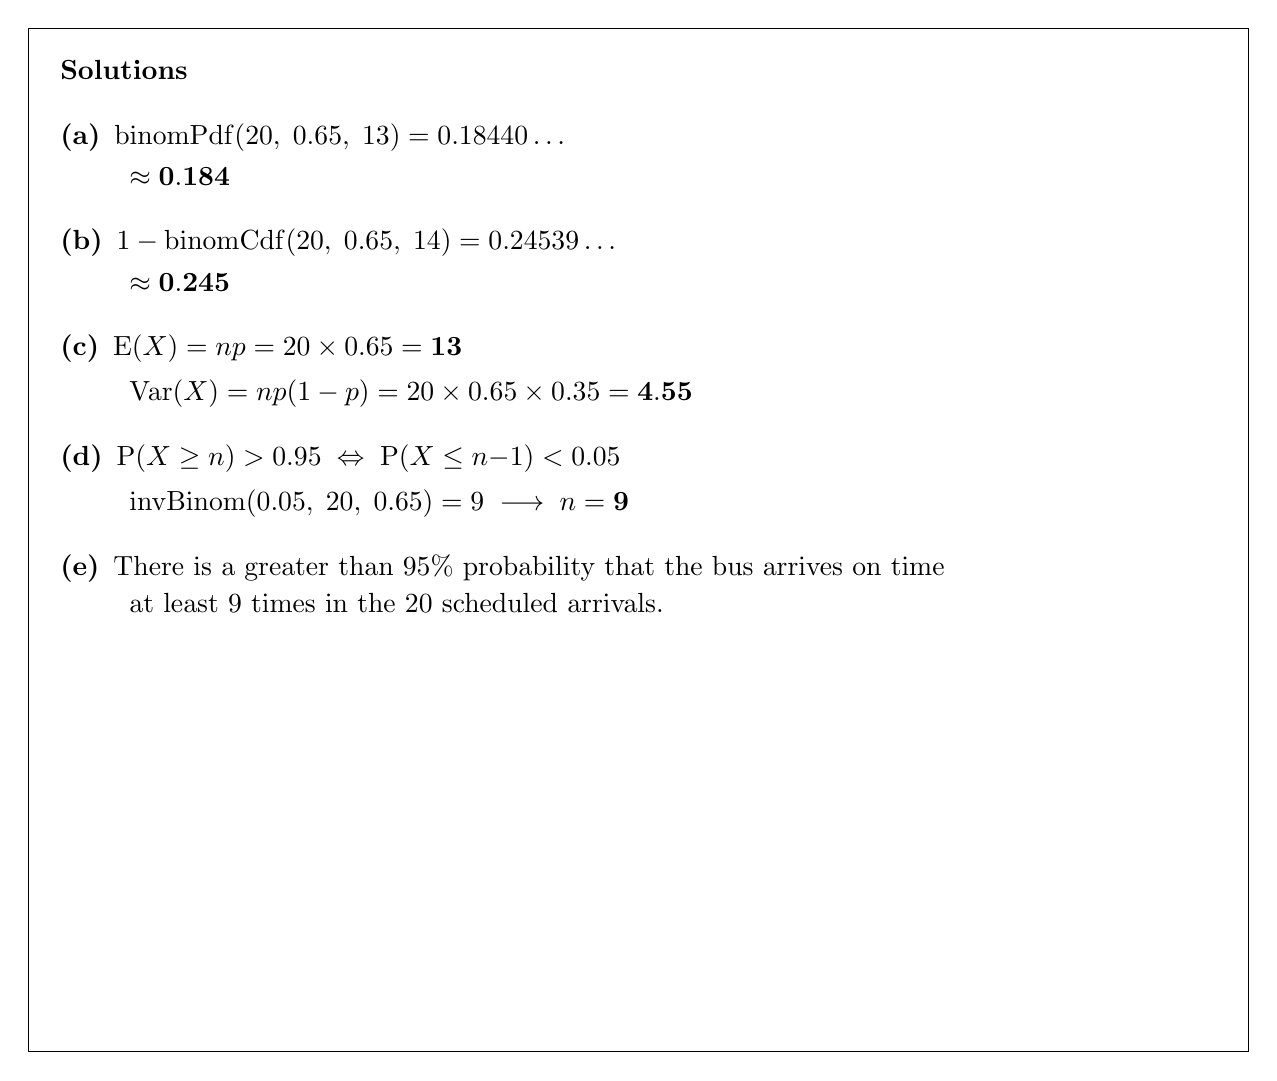
\begin{tikzpicture}
  \draw (0,0) rectangle (15.5,13);
  \node[anchor=north west, inner sep=0.40cm] at (0,13) {%
    \begin{minipage}[t]{14.7cm}%
      \textbf{Solutions}\\[0.4cm]
      %--- (a) ---
      \textbf{(a)}\enspace $\mathrm{binomPdf}(20,\;0.65,\;13) = 0.18440\ldots$\\[0.1cm]
      \hspace*{2.5em}$\approx \mathbf{0.184}$\\[0.4cm]
      %--- (b) ---
      \textbf{(b)}\enspace $1 - \mathrm{binomCdf}(20,\;0.65,\;14) = 0.24539\ldots$\\[0.1cm]
      \hspace*{2.5em}$\approx \mathbf{0.245}$\\[0.4cm]
      %--- (c) ---
      \textbf{(c)}\enspace $\mathrm{E}(X) = np = 20 \times 0.65 = \mathbf{13}$\\[0.15cm]
      \hspace*{2.5em}$\mathrm{Var}(X) = np(1-p) = 20 \times 0.65 \times 0.35 = \mathbf{4.55}$\\[0.4cm]
      %--- (d) invBinom ---
      \textbf{(d)}\enspace
        $\mathrm{P}(X \geq n) > 0.95
         \;\Leftrightarrow\;
         \mathrm{P}(X \leq n{-}1) < 0.05$\\[0.15cm]
      \hspace*{2.5em}$\mathrm{invBinom}(0.05,\;20,\;0.65) = 9
         \;\longrightarrow\; n = \mathbf{9}$\\[0.4cm]
      %--- (e) ---
      \textbf{(e)}\enspace There is a greater than 95\% probability that the bus arrives
      on time\\[0.05cm]
      \hspace*{2.5em}at least 9 times in the 20 scheduled arrivals.%
    \end{minipage}%
  };
\end{tikzpicture}

\end{enumerate}
\end{document}
